\chapter{Materiales y Herramientas}
%\vspace{-1cm}
En este capítulo se exponen los materiales utilizados para cada componente del sistema, las herramientas utilizadas para el modelado 3D del nano-espaciador, simulación de la transmisión de calor por conducción y simulación de transmisión de calor por radiación por campo cercano, y los motivos de uso de dichos materiales y herramientas.
\section{Materiales}
Se listan y desarrolla los materiales a utilizar para cada uno de los componentes del sistema TPV, incluyendo los criterios seguidos de su selección.
\subsection{Nano-espaciador}
El nano-espaciador es de Dióxido de Silicio ($SiO_2$) \cite{doi:10.1063/1.1141498}, un material que ha sido utilizado en varias ocasiones en sistemas de campo cercano de TPVs o TEC por ser un material cerámico con una baja conductividad térmica, buena resistencia ante choques de calor y alta fuerza de compresión. La conductividad térmica es menor a 10 W/m\textdegree C en el rango de temperatura de trabajo, entre 25 a 800\textdegree C.\\\\
A su vez se considera el $SiO_2$ con tres porosidades distintas, la primera es con una porosidad del 0\%, segundo con una porosidad del 25\% y tercero con una porosidad del 50\%, calculando la nueva conductividad térmica para los casos de porosidad distinta al 0\% según el modelo CP en \cite{ThermalConductivity_SiO2_2018}.

\subsection{Célula}
La célula es en una primera instancia de Silicio (Si) para la realización de unas pruebas de simulación iniciales, se utiliza Silicio para dichas pruebas por ser muy conocido y utilizado en la fabricación de células fotovoltaicas. En el resto de simulaciones se utiliza Germanio (Ge), que es un semiconductor como el Si pero que es capaz de absorber una mayor cantidad de radiación por tener una banda energética (Band Gap) de 0.66eV a 300K, a diferencia del Si que es unos 1.11eV a 300K. La capacidad de absorber más radiación es importante en la termofotovolaica porque la mayor cantidad de radiación es infrarroja.\\

También se utiliza el Ge por ser el material de las células termofotovoltaicas a disposición en el Instituto de Energía Solar (IES).
\subsection{Emisor}
Para el emisor se utilizan Silicio, Acero inoxidable 304L (SS) y Carburo de Silicio (SiC). Se utilizá Si para las pruebas de simulación iniciales para tener un punto de partida, para luego pasar al \textit{SS} por ser un material que se utiliza mucho en la industria, incluyendo al transporte, y por último el SiC que es una cerámica que ha se ha utilizado para el aumento de potencia de radiación en campo cercano, aunque es mayor para una capa fina de SiC cercano a la frecuencia de resonancia \cite{doi:Near_field_ThinFilm}.
\begin{figure}[H]
	\centering
		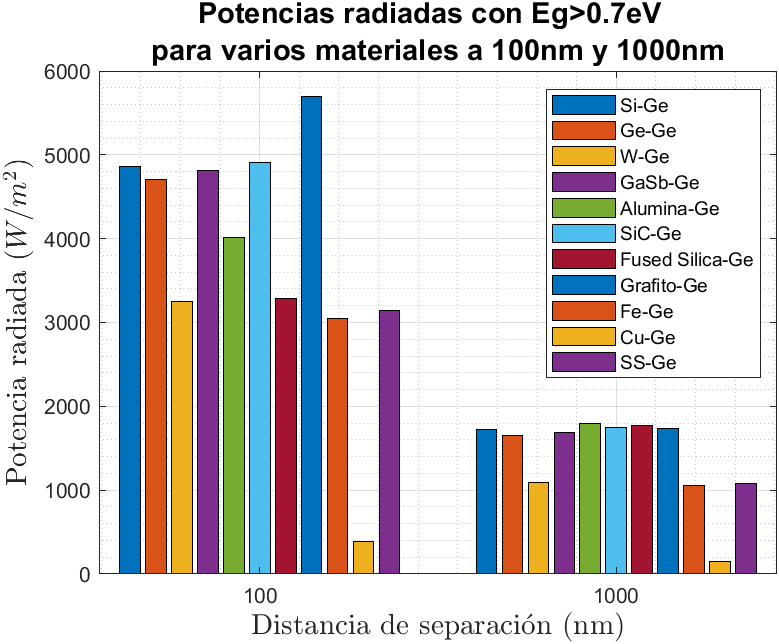
\includegraphics[width=0.6\textwidth]{figuras/rad_mat/EgRad.png}
	\caption{Potencias por unidad de área para una célula de Ge y diferentes materiales de emisor para un rango de longitudes de onda desde aproximadamente 0.2 $\mu m$ hasta 1.8 $\mu m$ (0.7 eV) con distancias de separación de 100nm y 1000nm según las ecuaciones de \cite{nfTPV_equations} implementadas en la calculadora de campo cercano.}
	\label{fig:EgRad}
\end{figure}
Se tomaron en cuenta otros materiales con mayor potencia de radiación (figura \ref{fig:EgRad}) o propiedades térmicas que han sido descartados por varias razones, entre ellas ser muy caros, tener baja potencia de radiación de campo cercano respecto a una célula de Ge, entre otros. %, similar conductividad térmica al SiC, Si o SS, punto de fusión menor o cercano a los 800\textdegree C, o por ser demasiado blandos. 
Dichos materiales son los siguientes:

\begin{itemize}
	\item \textbf{Antimoniuro de Galio (GaSb)}: Semiconductor con punto de fusión de 710\textdegree C que es menor a los 800\textdegree C que se encuentra el emisor, por lo cual no se puede utilizar porque empezará a pasar a estado líquido antes de llegar a la temperatura deseada.
	\item \textbf{Grafito}: es un material relativamente barato con una buena conductividad térmica, alto punto de fusión, pero es muy blando respecto al $SiO_2$, tiene como dureza máxima unos 50 HV (dureza Vickers) en comparación a la dureza del $SiO_2$ de unos 500 HV, por lo cual el nano-espaciador se hará paso por el emisor.
	\item \textbf{Tungsteno (W)}: El coste del material es medio, como máximo unos 56.4€/kg, su dureza Vickers es de unos 350 HV que es adecuada por no ser tan inferior a la del $SiO_2$, su conductividad térmica es más alta que la del nano-espaciador pero la potencia radiativa en campo cercano es baja, más cercana a la del acero.
	\item \textbf{Alumina ($Al_2O_3$)}: Es un material muy caro, aproximadamente 16000€/kg o más, disminuyendo considerablemente la viabilidad del sistema.
\end{itemize}

\section{Herramientas}

Los herramientas o programas utilizados durante el desarrollo del trabajo son variados y por diferentes motivos, a continuación se da una breve descripción y se explican los motivos de la utilización de cada programa.\\\\
Para la obtención de datos de los materiales se utilizan Granta EduPack 2021 R2, la página web Refractive Index y el resto de datos de los materiales que no se encuentren en dichas herramientas se obtienen de artículos de investigación. Para el modelado 3D se utiliza Autodesk Inventor 2021, para las simulaciones de la transmisión de calor por conducción se utiliza Autodesk CFD 2021, para la transmisión de calor por radiación se utiliza la Calculadora de campo cercano y para el análisis de datos se utiliza MATLAB.\\\\
Unas herramientas a destacar son TexStudio y TexnicCenter utilizadas para la redacción de este trabajo por la facilidad que presenta el escribir ecuaciones, actualizaciones de figuras y la menor necesidad de recursos que Word. También hay que destacar el uso de Git para el control de versiones del documento.\\
%%%  GRANTA EDUPACK 2021 R2
\subsection{Granta EduPack 2021 R2}
Programa desarrollado por la empresa Ansys que contiene varias bases de datos que recopila información sobre distintos materiales, teniendo un fácil acceso a la información básica de los mismos a través de una interfaz gráfica (GUI) y estando organizadas de manera específica para cada base de datos. Este programa está disponible en la versión de Windows 10 del escritorio remoto de la UPM.\\\\
La base de datos utilizada es la \textit{Level 3} de las avanzadas porque recopila los datos de todos los materiales necesarios, en la mayoría de los casos incluye la variación de algunas propiedades respecto a la temperatura, siendo principalmente necesaria la conductividad térmica del material respecto a la temperatura.\\\\
Dado la gran cantidad de datos a disposición y la facilidad de obtención de los datos de los materiales, especialmente los datos que están disponibles con la variación de la temperatura, se utiliza este programa.
%%%   REFRACTIVE INDEX
\subsection{Refractive Index}
Esta página web (https://refractiveindex.info) recopila de artículos científicos los índices de refracción (n) e índices de extinción (k) de diferentes materiales en diferentes rangos de longitudes de onda, teniendo a disposición hipervínculos a los artículos de donde se extrajo los datos y la opción de descargar dichos datos.\\\\
El motivos de su utilización son la facilidad para la obtención de los índices de refracción y extinción, necesarios para los cálculos del flujo térmico de radiación por campo cercano, y la disponibilidad de los artículos utilizados para contrastar los valores presentados.

%\subsection{Modelado 3D}
%Para el modelado 3D de cada componente del sistema (emisor, célula y nano-espaciador) se utiliza Autodesk Inventor 2021 por la facilidades que presenta autoDesk de utilizar los archivos de un programa de la misma compañía en otro programa para continuar con el estudio del sistema.ç
%%%  Autodesk INVENTOR 2021
\subsection{Autodesk Inventor Professional 2021}
Es un software de Diseño 3D Asistido por Ordenador (CAD 3D) que ofrece herramientas para el diseño de piezas, ensamblajes, mecanismos, documentación y simulación de los sistemas. También permite el utilizar herramientas de entorno añadidas para simulaciones más complejas, el fácil acoplamiento para el uso de otros programas de Autodesk y el uso de parámetros en el diseño y modelado de las piezas.
\begin{figure}[H]
	\centering
		
\includegraphics[width=3cm]{figuras/inventorpro.png}
	\caption{Icono de Autodesk Inventor Professional 2021}
	\label{fig:inventorpro}
\end{figure}
Se utiliza el programa para el modelado 3D de los nano-espaciadores, el emisor, la célula y el sistema TPV completo. Los motivos de utilización del programa son:

\begin{itemize}
	\item Licencia estudiantil facilitada por la Universidad Politécnica de Madrid (UPM).
	\item Menor consumo de recursos que otros programas de modelado 3D.
	\item No necesita una conexión constante a internet para su uso.
	\item Acoplamiento con Autodesk CFD, permitiendo el lanzar modelos de Inventor a CFD. 
\end{itemize}

%\subsection{Simulaciones de transmisión de calor por conducción}
%Para la simulación de transmisión de calor se usa el programa Autodesk Computational Fluid Dynamics (CFD), que aún ser usado principalmente para simulaciones con fluidos también permite simular solo transmisión de calor por conducción en sólidos y permite usar los diseños de Autodesk Inventor para simular, siendo fácilmente creado el provecto de CFD desde Inventor en la pestaña nueva de simulación, que se crea automáticamente con la instalación de CFD, y haciendo click sobre \textit{Active Model Assessment Tool}. Usándose exclusivamente para las simulaciones de conducción porque no puede simular la transmisión de calor por campo cercano.
\subsection{Autodesk CFD}
Es un software desarrollado por Autodesk que se usa para crear simulaciones computacional de la dinámica de fluidos para la predicción del comportamiento complejo de fluidos (líquidos y gases), el programa también simula la transmisión de calor por conducción en sólidos, convección en fluidos y de radiación con la ayuda de un medio fluido. \\
\begin{figure}[H]
	\centering
		
\includegraphics[width=3cm]{figuras/CFD.png}
	\caption{Icono de Autodesk CFD}
	\label{fig:CFD}
\end{figure}
Se utiliza el programa para las simulaciones de transmisión de calor por conducción en vez de el entorno Nastran de Inventor por las siguientes razones:
\begin{itemize}
	\item Utilización de escalas pequeñas de los parámetros de los materiales.
	\item Fácil control del mallado.
	\item Control de los pasos de la simulación, la frecuencia de guardado de datos y el número de iteraciones.
	\item Fácil obtención de los datos de los flujos de calor y las temperaturas del espaciador en formato CSV.
	\item Obtención de un modelo de simulación desde Autodesk Inventor,
\end{itemize}

\subsection{MATLAB}
MATLAB es un programa o plataforma de programación de \textit{MathWorks} que permite desarrollar cálculos numéricos, desarrollar algoritmos, analizar datos y crear modelos matemáticos de sistemas para cálculo o simulaciones utilizando su propio lenguaje de programación. A su vez, MATLAB proporciona una tienda de paquetes donde los usuarios puede subir aplicaciones desarrolladas en MATLAB que permiten aprovechar aún más los recursos del sistema y facilitar el trabajo, ya sea analizar datos, obtener modelos matemáticos, entre otros.\\
\begin{figure}[H]
	\centering
		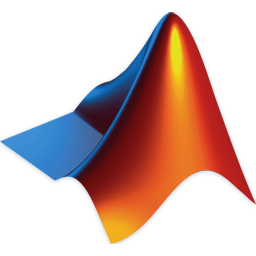
\includegraphics[width=3cm]{figuras/MatlabIcon.png}
	\caption{Icono de MATLAB}
	\label{fig:MatlabIcon}
\end{figure}
Se utiliza MATLAB para el análisis de los resultados obtenidos de las simulaciones de transmisión de calor por conducción y radiación, para realizar gráficas, para realizar cálculos y para desarrollar la aplicación de la calculadora de campo cercano. El principal motivo de usar MATLAB es porque el código principal de cálculo de transferencia de calor por radiación de campo cercano proporcionado está desarrollado en MATLAB.

\subsection{Calculadora de campo cercano}
Para las simulaciones de transmisión de calor por radiación de campo cercano entre dos placas paralelas de área infinita utilizando un código proporcionado que está escrito en MATLAB que cumple con las ecuaciones de campo cercano de \cite{nfTPV_equations} para dos placas planas gruesas y a partir de dicho código se desarrolla una aplicación en el App Designer de MATLAB para facilitar el proceso de calcular cualquier combinación de materiales para el emisor y la célula para ciertas distancias de separación. Se aprovecha la Toolbox Parallel Processing para realizar los cálculos con hilos y así disminuir los tiempos de simulación.\\\\
Los motivos que impulsaron para desarrollar la aplicación son el simplificar el proceso de simular la radiación por campo cercano para diferentes combinaciones de materiales y distancia de separación, y la obtención de la potencia total para el rango de longitudes de onda deseadas para todas las combinaciones.\\

La aplicación se divide en tres pestañas \textit{Potencia Radiada}, \textit{Potencia} y \textit{Materiales}. En cuanto se abre la aplicación se presenta abierta la pestaña de \textit{Potencia Radiada} (figura \ref{fig:pestana_PotenciaRadiada}), donde se seleccionan los materiales del emisor y el receptor, las distancias de separación de los cuerpos y la temperatura del emisor en grados Kelvin, ya que la del receptor es fija a 300K y no influye en los cálculos. También muestra la gráfica de los resultados obtenidos de la simulación para cualquier combinación excepto cuando se eligen varios materiales y un rango de distancias.\\ 
\begin{figure}[H]
	\centering
		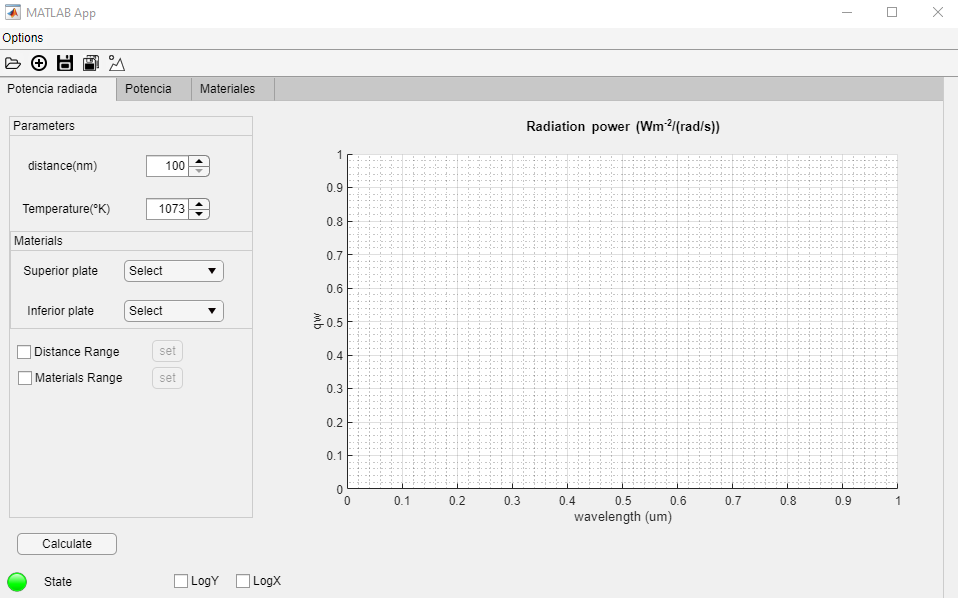
\includegraphics[width=0.80\textwidth]{figuras/pestana_PotenciaRadiada.png}
	\caption{Pestaña \textit{Potencia Radiada} de la calculadora de campo cercano}
	\label{fig:pestana_PotenciaRadiada}
\end{figure}
Para la selección del rango de los materiales se abre una nueva ventana de una GUI donde se utiliza dos árboles de casillas de selección para los materiales del emisor y el receptor del sistema de transmisión de calor por radiación de campo cercano (figura \ref{fig:ventana_mat}). Para la selección del rango de distancias se abre una nueva ventana de una GUI donde se el paso entre para variar las distancias límites es 100nm, las distancias máxima y mínima son 1000nm y 100nm (figura \ref{fig:ventana_dist}).Antes de realizar los cálculos se realiza una interpolación lineal de los valores de n y k de los materiales para que coincidan los puntos para cada longitud de onda.\\\\
\begin{figure}[H]%
\centering
\begin{subfigure}[b]{0.48\textwidth}
\centering
	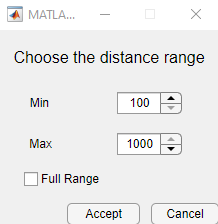
\includegraphics[width=0.75\textwidth]{figuras/pestana_Distancias.png}
	\caption{Ventana de selección de rango de distancias}%
	\label{fig:ventana_dist}%
\end{subfigure}
\hfill
\begin{subfigure}[b]{0.48\textwidth}
\centering
	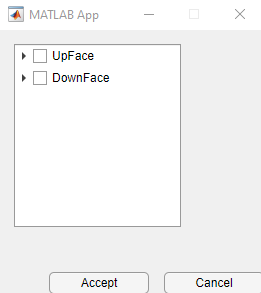
\includegraphics[width=0.75\textwidth]{figuras/pestana_Elegirmateriales.png}
	\caption{Ventana de selección de materiales}%
	\label{fig:ventana_mat}%
\end{subfigure}
\caption{(\subref{fig:ventana_dist}) Ventana para la selección del rango de las distancias de separación entre el emisor y el receptor. (\subref{fig:ventana_mat}) Ventana para la selección de los materiales para el emisor y el receptor.}%
\label{fig:ventanas_d_mat}%
\end{figure}
La pestaña de \textit{Potencia} (figura \ref{fig:pestana_Potencia})contiene una calculadora para pasar de electrón-voltios a longitud de onda y viceversa, unos campos para controlar el rango de longitudes de onda para realizar la integral de la potencia radiada y una gráfica para mostrar los resultados obtenidos de integrar. La integral se realiza por el método del trapezoide. Los resultados obtenidos de la potencia, los de la potencia radiada o ambos se pueden guardar en un archivo excel.
\begin{figure}[H]
	\centering
		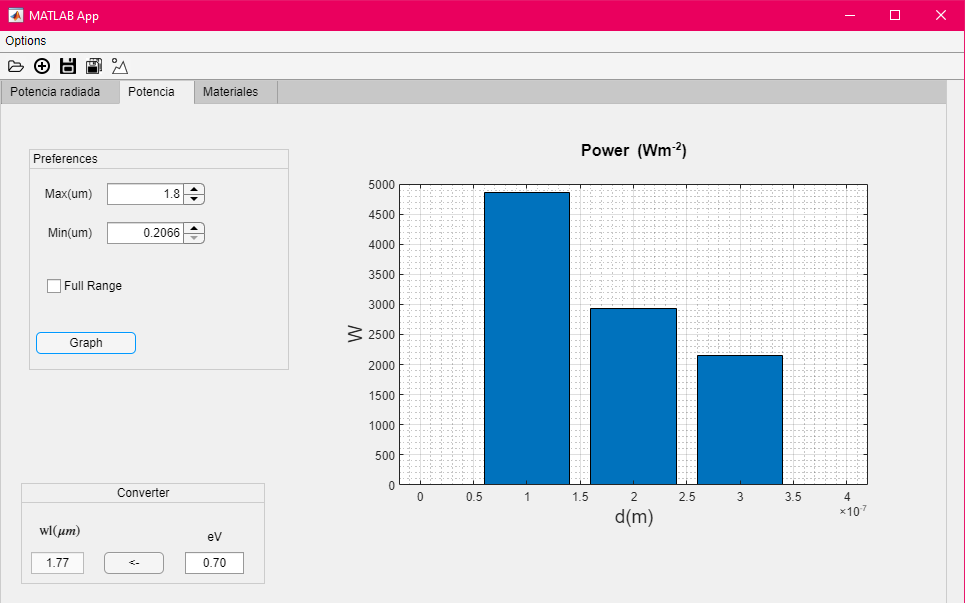
\includegraphics[width=0.70\textwidth]{figuras/pestana_Potencia.png}
	\caption{Pestaña de la Potencia}
	\label{fig:pestana_Potencia}
\end{figure}
La pestaña de \textit{Materiales} se usa para observar en una tabla o gráfica, según la pestaña interna seleccionada, los valores de n y k del material seleccionado en la lista de la izquierda, como se puede observar en la figura \ref{fig:pestana_materiales}.
\begin{figure}[H]
	\centering
		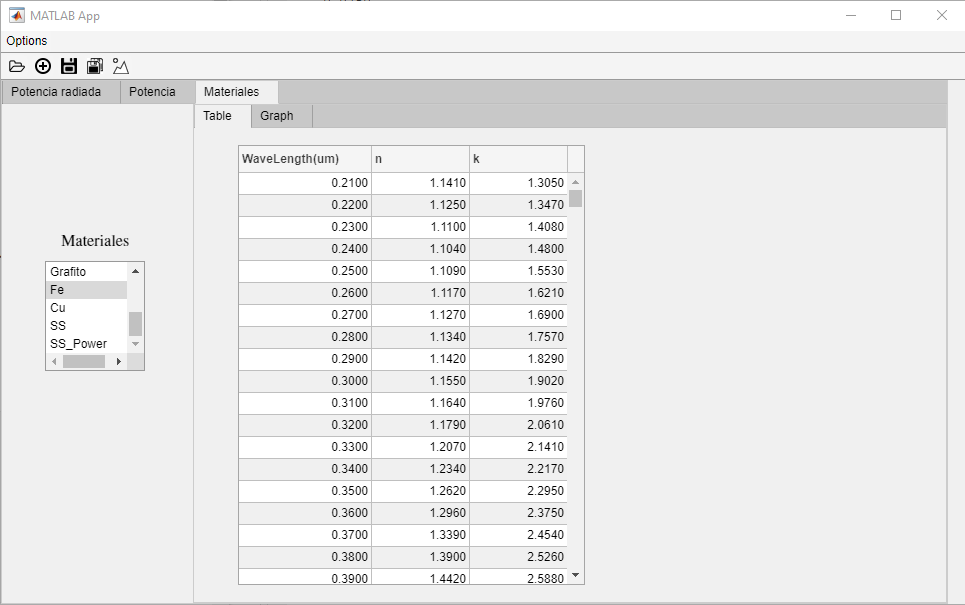
\includegraphics[width=0.70\textwidth]{figuras/pestana_materiales.png}
	\caption{Pestaña de los datos de n y k  de los materiales disponibles}
	\label{fig:pestana_materiales}
\end{figure}
Para obtener una mejor fidelidad de los resultados de la simulaciones se limita el rango de los datos dentro de las longitudes de onda que comparten todos los materiales del conjunto que se va a simular, teniendo en cuenta que para el acero inoxidable se extrapolaron los datos de $n$ y $k$ desde 1.2 $\mu m$ hasta los 1.8$\mu m$ que equivalen a 0.7 eV.\\\\
Cabe destacar que la aplicación sigue en fase de desarrollo y todavía no se ha terminado de agregar todas las funcionalidades deseadas, y arreglar los bugs que todavía tiene.